% Chapter Template

\chapter{Physical phenomena of fluid dynamics} % Main chapter title

\label{Chapter2} % Change X to a consecutive number; for referencing this chapter elsewhere, use \ref{ChapterX}

\lhead{Chapter 2. \emph{Physical fluid dynamics}} % Change X to a consecutive number; this is for the header on each page - perhaps a shortened title

%----------------------------------------------------------------------------------------
%	SECTION 1
%----------------------------------------------------------------------------------------

\section {Physical introduction}

In this chapter the physical basics of fluid dynamics shall be introduced and explained. Since the focus of this Chapter is to give the novice reader a good understanding  of the underlying physical and mathematical terms of CFD, at first specific physical phenomenon of fluids are presented and illustrated in detail before slowly moving to the realms of mathematics in this Chapter and the following to further describe these phenomena. We start with the explanation of several important terms of the field and then continue with the governing equations of fluid dynamics by explaining them with the simpler Euler equations in the next Chapter. Afterwards the Navier-Stokes equations are presented as an extension of the Euler equations. In Chapter \ref{Chapter3}  the given equations are explained in more detail from the mathematical and numerical view.



\section{Fluid dynamics terminology}
First of all the most important terms in fluid dynamics are presented and illustrated. However the field of
CFD is very large and not all terms can be coverted. This Chapter focuses on the terms that are necessary to understand the following Chapters. For further reading \citep{Hughes1999} \citep{Potter2009} and \citep{Biringen2011} are recommended.

\section{Internal Flows}

\section{External Flows}
A external flow is considered to be a fluid flow that takes places around or outside of a certain geometry body. Examples of such flow occur around
an airfoil of a airplane, as illustrated in Figure \ref{fig:ExternalFlowAirfoil}  Fluid Mechanics Dem Page 67 Figure 3.6 modified


\begin{figure}[htp]
\centering
\includegraphics[scale=0.50]{Figures/ExternaFlowModified.png}
\caption{External flow on around airfoil}
\label{fig:ExternalFlowAirfoil}
\end{figure}

For further reading on internal and external flows please refer to \cite{Hirsch2007}.

\section{Unsteady flow}


\section{Incompressible fluids}
\label{sec:incompress_fluid}



\section{Inviscid flow}
\label{sec:invisicid_flow}
The ideal flow also known as


%Newtonian fluids

\section{Laminar flow}

If viscosity can be considered important in the modelling of the fluid flow, 
A laminar flow is one in which no or relatively neglible amounts of fluid particles mix together in the course of the flow direction. A illustration
of this circumstance can be viewed in Figure \ref{fig:LaminarFlowPlain}. The coloured streams represent the flow of one fluid along a short pipe. The motion
of the coloured streams remains smooth and uniform without random mixing of colours. The fluid travels smoothly along regular paths and the different coloured
fluid layers slide over each other without interception.


\begin{figure}[htp]
\centering
\includegraphics[scale=0.05]{/home/nabladev/Dropbox/____SEMINAR_CFD/text/Figures/laminarflow_plain.jpeg}
\caption{Laminar flow}
\label{fig:LaminarFlowPlain}
\end{figure}

\begin{figure}[htp]
\centering
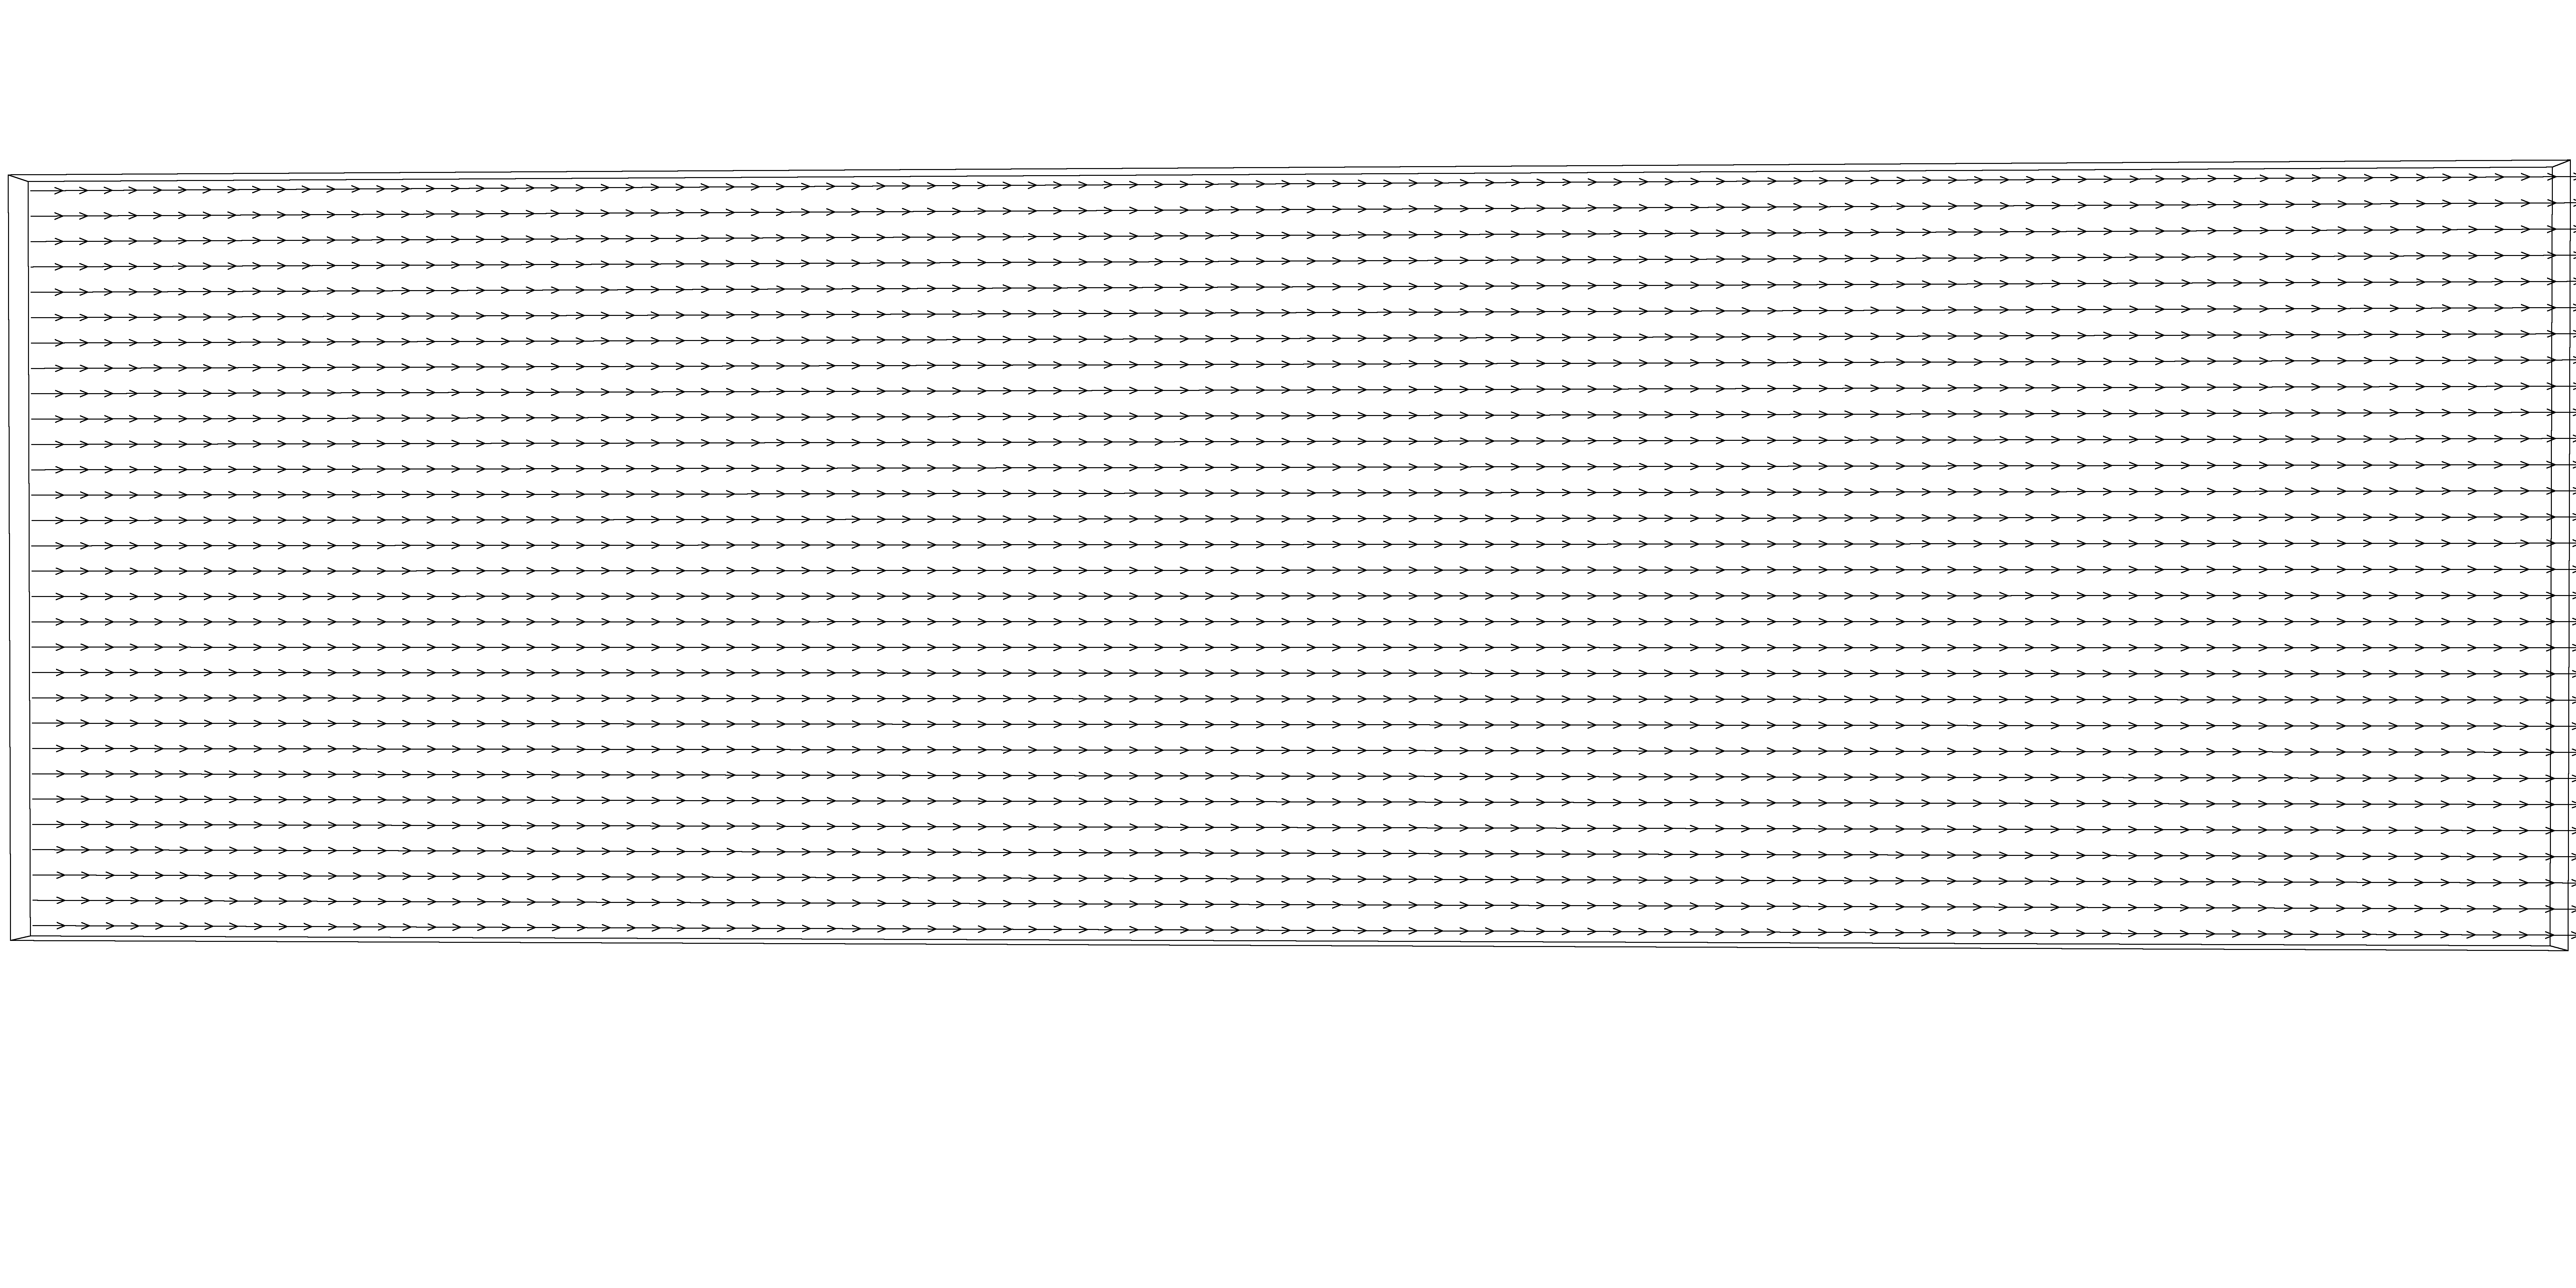
\includegraphics[scale=0.05]{/home/nabladev/Dropbox/____SEMINAR_CFD/text/Figures/laminarflow_vectors.png}
\caption{Velocity field of the laminar flow}
\label{LaminarFlowVector}
\end{figure}



\section{Turbulent flow}

Turbulent flow can be considered the opposite of laminar flow. Heavy mixing of fluid particles takes place in a turbulent flow. Important to note is that turbulence is a property of the the fluid flow not of the fluid itself. The motion of the flow itself and
each individual particle can be very noisy and random. In Figure \ref{fig:TurbulentFlowPlain} after a short period of uniform laminar flow the colour streams break up
and become turbulent. There is heavy mixing of colour noticeable and the fluid's path become chaotic. This is due to the viscosity of the fluid itself and also the lenght itself of geometry the fluid
flows along. In general any kind of random variations in a flow's quantities is considered to be turbulent. In Figure \ref{fig:TurbulentFlowVector} this is the velocity: The random fluctuation of the velocity can be seen at a certain moment. the All this factors are represented with the Reynolds number \textbf{Re} which makes it possible to determine if a flow is likely to be laminar or
turbulent. Important ist to understand the difference between fluids and flow since 


\begin{figure}[htp]
\centering
\includegraphics[scale=0.05]{/home/nabladev/Dropbox/____SEMINAR_CFD/text/Figures/turbulentflow_plain.jpeg}
\caption{Turbulent flow}
\label{fig:TurbulentFlowPlain}
\end{figure}



\begin{figure}[htp]
\centering
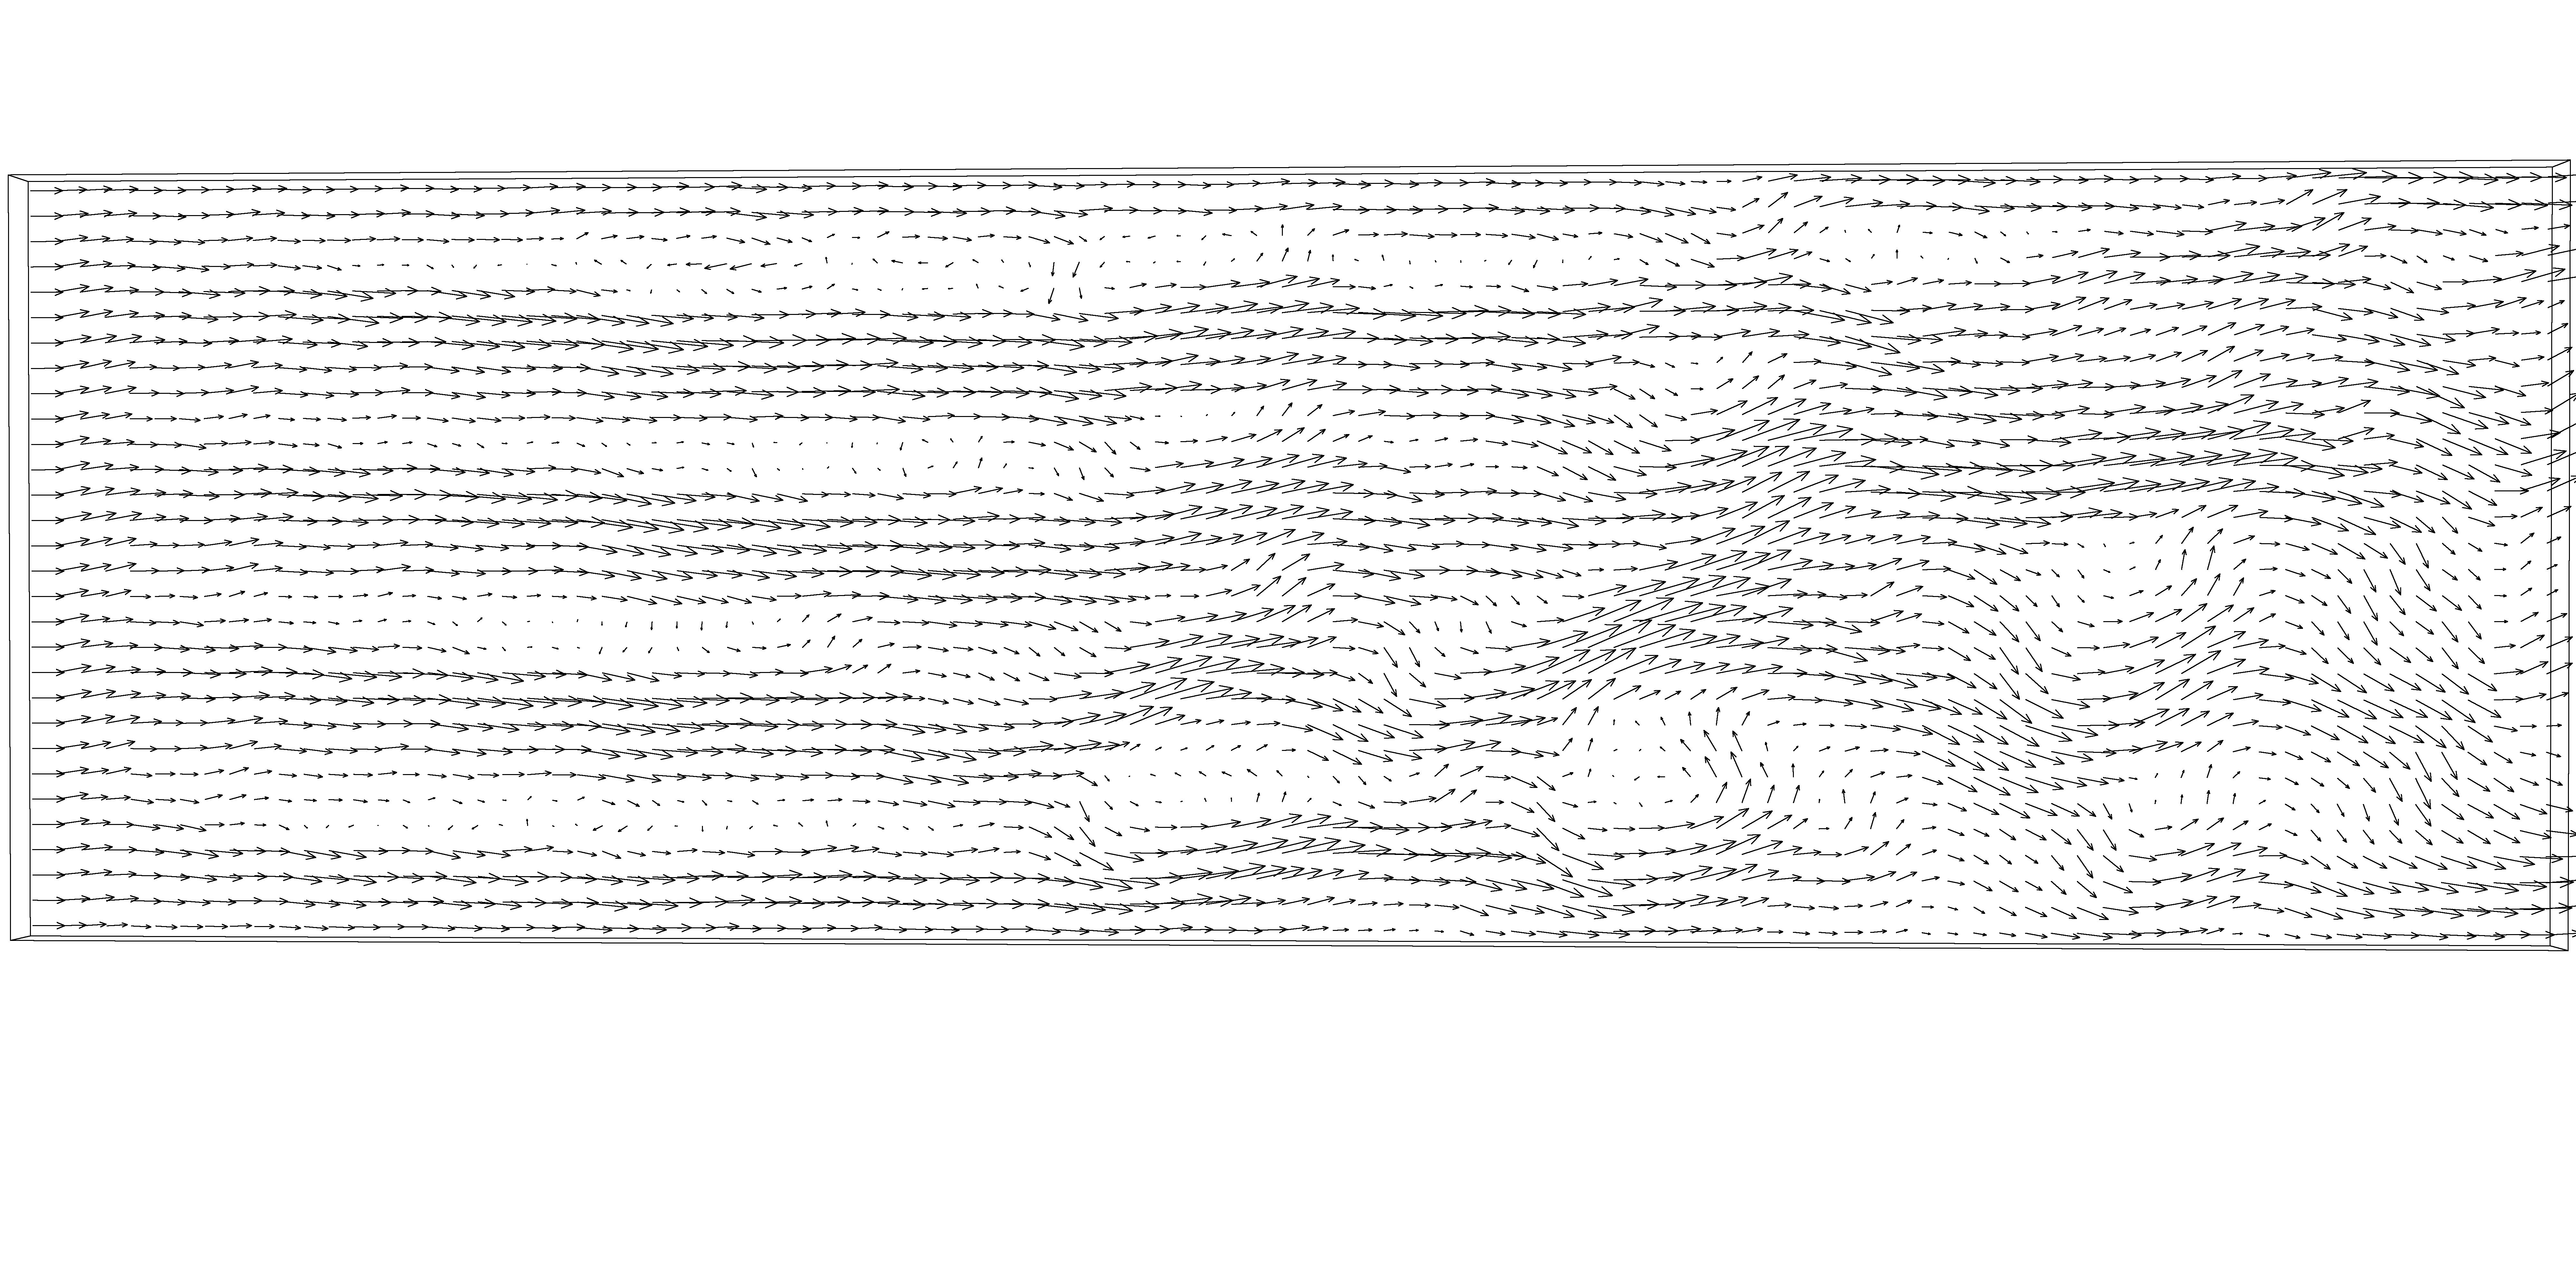
\includegraphics[scale=0.05]{/home/nabladev/Dropbox/____SEMINAR_CFD/text/Figures/turbulentflow_vectors.png}
\caption{Velocity field of the turbulent flow}
\label{fig:TurbulentFlowVector}
\end{figure}

\subsection{Reynolds number}

The dimensionless Reynolds number is used to relate inertial forces to viscous forces in a fluid flow. It can be determined as follows and its value helps to estimate if a flow is more likely to be laminar or turbulent. 


\[
Re = 
\frac {VL}{\nu} 
\]


With V denoting the average velocity of the fluid inside or outside the geometry, L
as the characteristic linear dimension or length of the fluid flow (e.g. travelled distance of a fluid) and \(\nu\) as the kinematic viscosity of the fluid.

The linear dimension L varies greatly between different geometry types and is subject to engineering convention. For instance not the lenght but the diameter of a pipe is used when computing Reynolds numbers for the internal flow in respective geometry today. Therfore when comparing Reynolds number as follows one always needs to consider the geometry for which it was computed and can not easily compare Reynolds numbers of different geometry classes.

Laminar flow occurs in general when the viscous forces are dominant, hence the Reynolds number needs to be low. Turbulent flows occur when the inertial forces are dominant. As rule of thumb if the Reynolds number is relatively large the flow is likely to be turbulent (Re > 4000), accordingly small numbers are likely to imply a laminar flow (Re < 2100).
The term "relative" means that the seperation betweeen large and small Reynolds numbers is dependend on the \emph{critical} Reynolds number. This critical Reynolds number determines the thresholds and is geometry dependend.
In 

\begin {table}[htp]
\begin{tabular}{lll}

\end{tabular}
\caption{Table of critical Reynolds numbers}
\end {table}




